\documentclass{article}
\usepackage[utf8]{inputenc}
\usepackage[hungarian]{babel} % set the language

\usepackage{lipsum}
\usepackage{graphicx} % for the includegrapichs
\usepackage{titling}

\usepackage{fancyhdr} % for the header on the first page
\usepackage{pdfpages} % to include pdf
%\usepackage{structuralanalysis} % for the figures



\begin{document}
	
	\begin{titlepage}
		\setlength{\headheight}{20pt}
		\lhead{
\includegraphics[height=1cm]{logo_aut.png}\\Elektrotechnika Csoport}
		\rhead{\large{\textbf{Analóg elektronika}}\\
			BMEVIAUA009}
		%\vspace{15cm}
		\title{\huge Házi feladat\\
			\Large Erősítő tervezés, áramkör szimuláció}
		\author{Tar Dániel\\GUTOY7}
		\date{\today}
		\maketitle
		\pagenumbering{gobble}
		\thispagestyle{fancy}
		
		\begin{figure}
			\begin{center}
				
\includegraphics[height=2cm]{logo_bme_kicsi.eps}
			\end{center}
		\end{figure}
		
	\end{titlepage}
	\newpage
	
	
	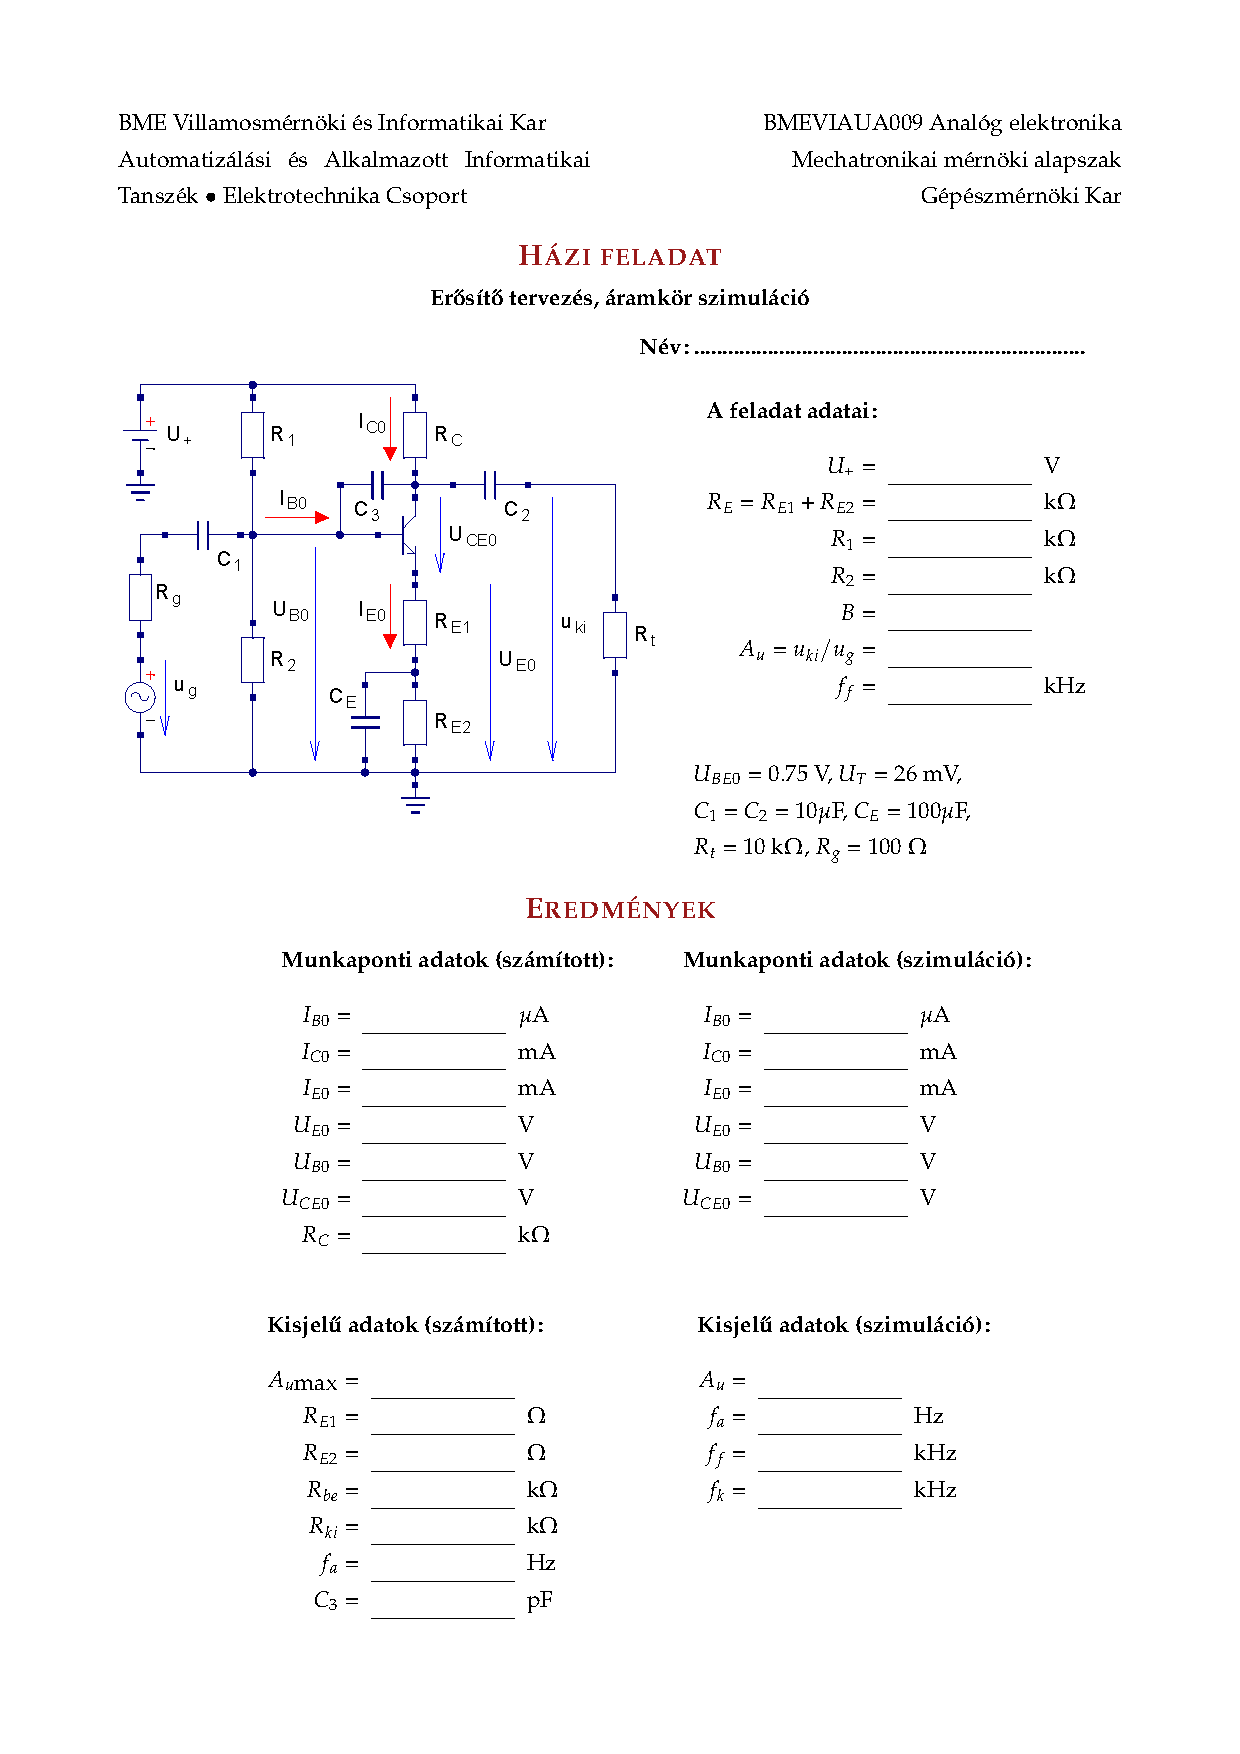
\includepdf[pages=1]{hf-2017-18-2.pdf} % insert the exercise description
	
\end{document}
